\documentclass[12pt,a4paper]{article}

\usepackage[utf8]{inputenc}
\usepackage[T1]{fontenc}
\usepackage[french]{babel}
\usepackage{geometry}
\usepackage{setspace}
\usepackage{hyperref}
\usepackage{xcolor}
\usepackage{booktabs}
\usepackage{array}
\usepackage{enumitem}
\usepackage{listings}
\usepackage{longtable}
\usepackage{graphicx}
\usepackage{caption}
\usepackage{subcaption}
\usepackage{tikz}
\usetikzlibrary{positioning,arrows.meta}

\geometry{margin=2.5cm}
\onehalfspacing
\setcounter{tocdepth}{2}

\hypersetup{
    colorlinks=true,
    linkcolor=black,
    urlcolor=blue,
    citecolor=black
}

\definecolor{codegray}{RGB}{245,245,245}
\definecolor{codeborder}{RGB}{220,220,220}

\lstdefinestyle{pythonstyle}{
    language=Python,
    backgroundcolor=\color{codegray},
    basicstyle=\ttfamily\small,
    frame=single,
    rulecolor=\color{codeborder},
    breaklines=true,
    showstringspaces=false,
    tabsize=4
}

\title{CondruLytics\\Analyse et structuration des resultats du Challenge Condrusien}
\author{Nom de l'etudiant : \underline{\hspace{6cm}}}
\date{Annee academique : \underline{\hspace{4cm}}}

\begin{document}

\pagenumbering{gobble}
\begin{titlepage}
    \centering
    \vspace*{1.5cm}

    
\includegraphics[height=4cm]{./unamur.png}\\[0.4cm]
    {\Large \textbf{Université de Namur}}\\[0.1cm]
    {\large \textbf{Faculté d'Informatique}}\\[1.8cm]

    {\Large \textbf{IEDC001 – Projet individuel}\par}
    \vspace{1.2cm}

    {\Huge \textbf{CondruLytics}\par}
    \vspace{0.5cm}
    {\Large Analyse, prédiction et visualisation des résultats \\ du Challenge Condrusien \\ de 2006 à 2025\par}

    \vfill

    \begin{tabular}{rl}
        Etudiant : Mestré Michaël \\
        Professeur : Frénay Benoît \\
        Année academique : 2025-2026 \\
    \end{tabular}

    \vfill

    {\large \today\par}
\end{titlepage}

\pagenumbering{roman}
\tableofcontents
\newpage
\pagenumbering{arabic}

\section{Introduction}

Le projet \textit{CondruLytics} a pour objectif de transformer des résultats historiques des courses du \textbf{Challenge Condrusien}  en un jeu de données exploitable pour l'analyse, la visualisation et la modélisation. Les données de départ sont les différents classements au format PDF, publiés sur plusieurs années et selon des formats variables. Cette hétérogenéité rend nécessaire la mise en place d'un pipeline capable d'extraire les informations, de les harmoniser et de les stocker dans une base de données qui représentera la source stable pour la suite des analyses.

Le projet couvre les principales étapes d'un pipeline de données : extraction des fichiers, parsing des PDF, consolidation, nettoyage, chargement dans une base PostgreSQL, création de variables, apprentissage automatique pour prédire le temps des coureurs sur différentes courses et enfin visualisation interactive via le framework Python Streamlit \footnote{\url{https://streamlit.io}}.

\subsection{Contexte}

Le \textbf{Challenge Condrusien} \footnote{\url{https://challengecondrusien.com}} est un challenge de course à pied amateur sur routes et chemins vallonés qui regroupe une vingtaine d'organisation chaque année dans le Condroz liégeois. Chaque organisation propose différentes distances: une petite sous les 7km, une longue entre 10 et 17km et parfois une version trail de plus de 20km. Les classements contiennent notamment le nom des coureurs, leur position générale, leur catégorie, leur temps, leur club, la distance de la course et la date de l'épreuve. Les fichiers ZIP de départ proviennent de la page officielle des archives du Challenge Condrusien \footnote{\url{https://challengecondrusien.com/archives/}}. Les données d'archives couvrent la periode 2006-2025 à l'exception de l'année 2020 en raison de la pandémie de COVID-19.

La difficulté principale provient du fait que les classements ne suivent pas un format unique. Les PDF présentent des structures differentes : colonnes absentes, ordre variable des champs, présence ou non du numero de dossard, informations de course encodées dans le texte, ou encore changements de mise en page selon les années. Le projet répond a cette contrainte par l'utilisation de plusieurs parseurs spécialisés. Après cette étape d'extraction, les données sont nettoyées pour harmoniser les catégories, normaliser les temps et corriger les erreurs d'extraction. Le format des noms des coureurs sont strandardisés et certaines erreurs de saisie sont corrigées. La base de données relationnelle créée permet ensuite de structurer les données pour des analyses, des expérimentations de modélisation et différentes visualisations interactives.

\subsection{Objectifs}

Les objectifs du projet peuvent être regroupés selon les grands axes suivants:

\begin{enumerate}[label=\arabic*.]
    \item \textbf{Construire un jeu de données fiable} a partir de fichiers PDF historiques.
    \item \textbf{Harmoniser les informations} relatives aux coureurs, aux courses, aux catégories et aux performances.
    \item \textbf{Mettre en place une base de données stable} permettant de consulter les résultats, les coureurs et les courses.
    \item \textbf{Préparer des variables de modélisation} afin d'analyser l'évolution des performances et d'expérimenter des approches prédictives, notamment l'estimation du temps probable d'un coureur sur une course déjà présente dans l'historique mais qu'il n'a pas lui-même courue.
    \item \textbf{Créer des visualisations interactives} pour permettre aux coureurs d'explorer les données, leur progression, la prédiction des résultats.
\end{enumerate}

\subsection{Etapes}

Les objectifs précédents se traduisent en un pipeline de traitement structuré. Le projet part de fichiers d'archives, puis les transforme en une base exploitable pour l'analyse, la modélisation et la visualisation. La figure~\ref{fig:demarche-generale} résume les différentes étapes.

\begin{figure}[h!]
    \centering
    \resizebox{\textwidth}{!}{%
    \begin{tikzpicture}[
        flowstep/.style={
            draw,
            rounded corners=2pt,
            fill=gray!8,
            align=center,
            text width=3.1cm,
            minimum height=1.2cm,
            font=\small
        },
        dbstep/.style={
            draw,
            rounded corners=2pt,
            fill=blue!8,
            align=center,
            text width=3.2cm,
            minimum height=1.2cm,
            font=\small
        },
        modelstep/.style={
            draw,
            rounded corners=2pt,
            fill=green!8,
            align=center,
            text width=3.2cm,
            minimum height=1.2cm,
            font=\small
        },
        arrow/.style={-{Latex[length=3mm]}, thick}
    ]
        \node[flowstep] (archives) {Archives ZIP\\et fichiers PDF};
        \node[flowstep, right=0.8cm of archives] (parsing) {Parsing\\des classements};
        \node[flowstep, right=0.8cm of parsing] (cleaning) {Nettoyage\\et harmonisation};
        \node[dbstep, right=0.8cm of cleaning] (database) {DB PostgreSQL};

        \node[modelstep, below=1.4cm of database] (features) {Feature engineering};
        \node[modelstep, left=0.8cm of features] (modeling) {Prédictions};
        \node[flowstep, left=0.8cm of modeling] (streamlit) {Application Streamlit};

        \draw[arrow] (archives) -- (parsing);
        \draw[arrow] (parsing) -- (cleaning);
        \draw[arrow] (cleaning) -- (database);
        \draw[arrow] (database) -- (features);
        \draw[arrow] (features) -- (modeling);
        \draw[arrow] (modeling) -- (streamlit);
        \draw[arrow] (database.south west) -- ++(0,-0.7) -| (streamlit.north);
    \end{tikzpicture}%
    }
    \caption{Schéma des étapes du projet.}
    \label{fig:demarche-generale}
\end{figure}

Les sections suivantes détaillent chacune de ces étapes.

\clearpage

\section{Extraction des données et préparation}

\subsection{Architecture générale}

Le projet est organisé sous forme de modules Python séparés par responsabilité. Cette décomposition facilite la maintenance et rend le pipeline reproductible.

\begin{longtable}{p{5.2cm}p{8.8cm}}
\toprule
\textbf{Module} & \textbf{Role principal} \\
\midrule
\texttt{src/extraction} & Décompression des archives ZIP contenant les classements bruts. \\
\texttt{src/parsing} & Extraction des données depuis les fichiers PDF. \\
\texttt{src/cleaning} & Nettoyage, normalisation et correction des données extraites. \\
\texttt{src/loading} & Définition du schema relationnel et chargement vers PostgreSQL. \\
\texttt{src/utils} & Centralisation des fonctions utilitaires globales. \\
\texttt{src/feature\_engineering} & Création de variables derivées pour l'analyse avancée et la modélisation. \\
\bottomrule
\end{longtable}

Un système de logging est mis en place pour suivre l'exécution du pipeline et identifier les éventuelles erreurs ou anomalies.

Le point d'entrée principal est le fichier \texttt{src/pipeline.py}. Celui-ci permet d'exécuter l'ensemble du pipeline ETL ou une étape spécifique via l'argument \texttt{--step}. Les étapes disponibles sont : \texttt{unzip}, \texttt{parse}, \texttt{build}, \texttt{clean} et \texttt{load}.

Les données intermédiaires sont stockées au format Parquet dans \texttt{data/processed/parquet}, ce qui permet de conserver une trace des résultats de chaque étape et de faciliter les reprises en cas d'erreur.

Les autres modules sont exécutés de manière séparée pour des tâches spécifiques, notamment la création de variables, ce qui rend le projet plus flexible et modulaire.

\subsection{Extraction des fichiers ZIP}

La première étape consiste a décompresser les archives ZIP situées dans \texttt{data/raw/zip}. Ces archives ont été récupérées depuis la page officielle des archives du Challenge Condrusien \footnote{\url{https://challengecondrusien.com/archives/}}, qui centralise les classements historiques disponibles. Le module \texttt{extraction.unzip} parcourt récursivement les archives, extrait les fichiers et produit un rapport de synthèse. Ce rapport indique le nombre de fichiers extraits, le nombre de fichiers ignorés car déja présents et le volume total traité.

\subsection{Parsing des fichiers PDF}

Le parsing est l'étape la plus sensible du projet. Les fichiers PDF sont convertis en tableaux de données grâce a la bibliothèque \texttt{pdfplumber}. Le projet utilise un patron de conception de type \texttt{Strategy} et un \texttt{ParserFactory}, choisit automatiquement le parseur adapté au fichier analyse.

Les stratégies implémentées permettent d'extraire toutes les données sur la plage de temps analysée et sont les suivantes :

\begin{itemize}
    \item \texttt{Parser2006\_2007}, adapté aux classements des années 2006 et 2007 ;
    \item \texttt{Parser2008\_2016}, adapté aux formats intermédiaires sans URL dans le texte ;
    \item \texttt{Parser2017\_2024}, adapté aux formats plus récents contenant des marqueurs web ;
    \item \texttt{Parser2025}, adapté aux classements produits par le chronometreur \texttt{Goal Timing}.
\end{itemize}

Chaque parseur extrait les champs principaux suivants : position, nom du coureur, club, sexe, catégorie, position dans la catégorie, temps, nom de la course, date et distance. Un identifiant de course, appelé \texttt{racekey}, est ensuite construit a partir du nom de la course, de la date et de la distance.

Le service de parsing traite les fichiers en parallèle avec \texttt{ThreadPoolExecutor}. Il génère également un rapport indiquant le statut de chaque fichier : succès, fichier ignoré, erreur ou différence entre le nombre de participants attendu et le nombre de lignes parsées.

Pour chaque fichier traité, un fichier Parquet est produit dans \texttt{data/processed/parquet} avec les données extraites. Ces fichiers intermédiaires sont ensuite utilisés pour les étapes suivantes du pipeline.

\subsection{Consolidation}

Apres le parsing, les fichiers Parquet intermédiaires sont consolidés dans un dataset unique. Cette étape concatène les résultats disponibles dans \texttt{data/processed/parquet}, supprime les éventuels doublons sur base de \texttt{racekey} et du nom du coureur, puis écrit le fichier \texttt{data/processed/results.parquet}.

\subsection{Nettoyage et harmonisation}

Le nettoyage est effectué par le module \texttt{cleaning.clean}. Il vise a rendre les données homogènes malgré les variations historiques de format. Les principales opérations sont :

\begin{itemize}
    \item harmonisation des catégories ;
    \item normalisation des temps au format \texttt{HH:MM:SS} puis conversion en secondes ;
    \item correction manuelle de certaines courses dont le nom ou la distance est mal extrait ;
    \item suppression de noms de coureurs invalides ou non exploitables ;
    \item correction ponctuelle de données coureurs connues ;
    \item normalisation des noms des coureurs afin de reduire les doublons ou erreurs orthographiques.
\end{itemize}

Une partie complexe du nettoyage concerne la correction du nom des coureurs. Dans les classements historiques, une même personne peut apparaître sous plusieurs formes : inversion du nom et du prénom, accentuation différente, caractères parasites, espaces multiples, fautes de frappe ou variations dues à l'extraction PDF. Se limiter au nom brut risquerait donc de considérer une même personne comme plusieurs individus distincts.

Le module \texttt{cleaning.clean\_names} applique d'abord une normalisation des chaînes de caractères : passage en majuscules, suppression des caractères non alphabétiques (tirets, apostrophes) et réduction des espaces multiples. Cette opération crée une colonne \texttt{Nom\_clean}, utilisée comme base de comparaison.

La correction ne repose cependant pas uniquement sur la similarité du nom. Le code construit un profil par coureur a partir de plusieurs informations :

\begin{itemize}
    \item le nombre d'apparitions du nom dans les résultats ;
    \item le sexe majoritaire observé ;
    \item la vitesse moyenne du coureur ;
    \item l'ensemble des courses auxquelles le coureur est associé, pour les coureurs fréquents.
\end{itemize}

Cette logique permet d'éviter des corrections trop agressives. Deux noms proches ne sont pas automatiquement fusionnés : ils doivent aussi être compatibles avec le profil sportif observé. Par exemple, deux profils de sexe différent ne sont pas rapprochés. De même, deux coureurs fréquents présents dans une même course ne peuvent pas être considérés comme une seule et même personne, car une personne ne peut pas avoir deux résultats distincts dans la même épreuve.

La méthode fonctionne en deux passes.

\begin{enumerate}[label=\arabic*.]
    \item \textbf{Première passe : coureurs fréquents entre eux.} Les coureurs apparaissant au moins trois fois sont comparés deux a deux. La similarité du nom est calculée avec un score de fuzzy matching à l'aide de la bibliothèque \texttt{RapidFuzz}. Ce score est combiné avec un score de proximité de vitesse. Le score final donne un poids dominant au nom, mais conserve une vérification par la performance. Si deux profils sont suffisamment proches, le nom le plus fréquent devient le nom corrigé. Cette première passe sur les coureurs fréquents permet de créer une base de noms fiables pour la suite du processus.
    \item \textbf{Deuxième passe : coureurs rares vs coureurs fréquents.} Après la première correction, les noms apparaissant moins de trois fois sont comparés aux coureurs fréquents. Pour limiter les comparaisons inutiles, une clé de blocage est créée a partir des premières lettres des parties du nom. Le fuzzy matching est ensuite appliqué uniquement à des candidats plausibles. Une correction est acceptée seulement si le score du nom et le score final dépassent des seuils élevés.
\end{enumerate}

Cette approche est volontairement prudente. L'objectif n'est pas de corriger tous les cas possibles, mais uniquement les cas pour lesquels le niveau de confiance est élevé. Cela signifie que certains doublons peuvent subsister, notamment lorsque le nom est très déformé, lorsque le coureur apparaît peu de fois ou lorsque son profil de coureur est insuffisant. En contrepartie, le risque de fusionner deux personnes différentes est réduit. Ce compromis est important pour ce travail d'analyse : il est préférable de conserver quelques doublons résiduels plutôt que de fusionner accidentellement des individus distincts.

La fin de l'étape de nettoyage produit \texttt{data/cleaned/results.parquet}. Il est néanmoins nécessaire de noter que les corrections n'écrasent pas les données brutes, une nouvelle colonne \texttt{Nom\_clean} est créée pour conserver le nom original et permettre de retracer les corrections appliquées.

\subsection{Modèle de données}

Les données nettoyées sont chargées dans une base de données PostgreSQL selon un schema en étoile simple compte tenu de la nature plate des données et des analyses prévues (figure~\ref{fig:schema-etoile}). Cette organisation reprend les principes classiques de la modélisation dimensionnelle, dans laquelle une table de faits porte les mesures et les clés étrangères vers les dimensions descriptives.

\begin{figure}[h]
    \centering
    \resizebox{\textwidth}{!}{%
    \begin{tikzpicture}[
        table/.style={
            draw,
            rounded corners=2pt,
            fill=gray!8,
            align=left,
            inner sep=7pt,
            text width=4.1cm,
            font=\small
        },
        fact/.style={
            draw,
            rounded corners=2pt,
            fill=blue!8,
            align=left,
            inner sep=7pt,
            text width=4.5cm,
            font=\small
        },
        link/.style={-{Latex[length=3mm]}, thick}
    ]
        \node[fact] (fact) {
            \textbf{fact\_results}\\
            \rule{\linewidth}{0.3pt}\\
            \texttt{result\_id}\\
            \texttt{runner\_id} (FK)\\
            \texttt{race\_id} (FK)\\
            position\\
            position\_category\\
            time\_sec \\ 
            speed\_kmh \\ 
            category\_seen\\
            category\_clean\\
            source\_file
        };

        \node[table, left=2.4cm of fact] (runner) {
            \textbf{dim\_runner}\\
            \rule{\linewidth}{0.3pt}\\
            \texttt{runner\_id} (PK)\\
            name\_origin\\
            name\_clean\\
            sex
        };

        \node[table, right=2.4cm of fact] (race) {
            \textbf{dim\_race}\\
            \rule{\linewidth}{0.3pt}\\
            \texttt{race\_id} (PK)\\
            \texttt{racekey}\\
            name\\
            distance\\
            date \\ 
            year
        };

        \draw[link] (fact.west) -- (runner.east);
        \draw[link] (fact.east) -- (race.west);
    \end{tikzpicture}%
    }
    \caption{Schéma en étoile utilisé pour structurer les résultats de courses.}
    \label{fig:schema-etoile}
\end{figure}

Bien que la catégorie puisse être considérée comme étant un attribut du coureur, elle est stockée dans la table de faits car elle peut varier d'une course à l'autre pour un même coureur (par exemple, un coureur peut être dans la catégorie "Senior" puis basculer dans la catégorie "Vétéran1" ensuite). De plus, cela permet de conserver une trace de la catégorie telle qu'elle a été observée dans les résultats, même si elle est parfois incohérente ou mal extraite.

Le schéma est ensuite étendu pour les besoins d'analyse et de prédiction. Pour rester dans une logique BI classique, cette extension prend la forme d'une seconde table de faits, \texttt{fact\_runner\_race\_analysis}. Elle a la même granularité que \texttt{fact\_results} : une observation correspond à un coureur sur une course. Elle partage donc les mêmes dimensions \texttt{dim\_runner} et \texttt{dim\_race}, mais elle n'est pas modélisée comme une table fille de \texttt{fact\_results}. La colonne \texttt{source\_result\_id} est conservée uniquement comme identifiant technique de traçabilité vers le résultat d'origine.

\begin{figure}[h!]
    \centering
    \resizebox{\textwidth}{!}{%
    \begin{tikzpicture}[
        dim/.style={draw, rounded corners, align=left, text width=4cm, minimum height=2.2cm, fill=gray!8, font=\small},
        analytic/.style={draw, rounded corners, align=left, text width=7.4cm, fill=green!8, inner sep=8pt, font=\small},
        link/.style={-{Latex[length=3mm]}, thick}
    ]
        \node[analytic] (analysis) {
            \textbf{fact\_runner\_race\_analysis}\\
            \rule{\linewidth}{0.3pt}\\
            \texttt{analysis\_id} (PK)\\
            \texttt{source\_result\_id}\\
            \texttt{runner\_id} (FK)\\
            \texttt{race\_id} (FK)\\
            actual\_position\\
            actual\_position\_category\\
            actual\_time\_sec\\
            actual\_speed\_kmh\\
            race\_month\\
            race\_dayofyear\\
            race\_participants\\
            race\_mean\_speed\\
            race\_std\_speed\\
            race\_median\_speed\\
            prior\_race\_count\\
            prior\_avg\_speed\\
            prior\_std\_speed\\
            prior\_best\_speed\\
            prior\_avg\_z\\
            prior\_std\_z\\
            prior\_best\_z\\
            recent\_speed\_roll3\\
            recent\_z\_roll3\\
            days\_since\_last\_race\\
            runner\_history\_years\\
            speed\_z\_race\\
            performance\_index\\
            target\_z\\
            predicted\_z\\
            predicted\_performance\_index\\
            predicted\_speed\_kmh\\
            predicted\_time\_sec\\
            abs\_error\_time\_sec\\
            split
        };

        \node[dim, right=3.2cm of analysis.north east, anchor=north west] (runner) {
            \textbf{dim\_runner}\\
            \rule{\linewidth}{0.3pt}\\
            \texttt{runner\_id} (PK)\\
            ...
        };

        \node[dim, below=1.2cm of runner] (race) {
            \textbf{dim\_race}\\
            \rule{\linewidth}{0.3pt}\\
            \texttt{race\_id} (PK)\\
            ...
        };

        \draw[link] (analysis.east) -- (runner.west);
        \draw[link] (analysis.east) -- (race.west);
    \end{tikzpicture}%
    }
    \caption{Extension analytique sous forme de seconde table de faits partageant les mêmes dimensions.}
    \label{fig:schema-etendu}
\end{figure}

Les prédictions à la demande, utilisées lorsqu'un coureur sélectionne une course qu'il n'a pas courue, ne sont pas stockées dans \texttt{fact\_runner\_race\_analysis}. Elles ne correspondent pas à un résultat observé dans l'historique. Elles sont donc calculées directement par l'application à partir du modèle entraîné.

Le chargement utilise des caches en mémoire pour un accès rapide et pour éviter de recréer plusieurs fois les mêmes coureurs ou les mêmes courses. Les résultats sont insérés par lots afin d'améliorer les performances d'écriture.

\subsection{Service PostgreSQL avec Docker}

Pour ce développement, la base de données PostgreSQL est fournie par un service Docker défini dans \texttt{docker/docker-compose.yml}. Ce fichier décrit un conteneur PostgreSQL nommé \texttt{condrulytics\_postgres}, expose le port \texttt{5432} et crée une base \texttt{condrulytics} avec un utilisateur dédié. Un volume Docker, \texttt{postgres\_data}, est associé au service afin de conserver les données entre deux redémarrages du conteneur. Cette approche permet d'utiliser rapidement une base de données locale, sans dépendre d'une installation PostgreSQL propre à une machine. Le code Python communique avec la base via SQLAlchemy et une configuration de connexion, ce qui signifie que la base Docker peut très facilement être remplacée par une base distante. 


\subsection{Feature engineering}

Le module \texttt{feature\_engineering.py} prépare un jeu de données destiné à deux objectifs : afficher l'évolution des performances d'un coureur dans l'interface finale et préparer une base de modélisation pour estimer un temps sur une course non encore courue. Cette étape est cruciale et ne doit pas utiliser des informations futures pour décrire un coureur au moment d'une course donnée, ce qui serait une fuite de données (\textit{data leakage}) et rendrait les modèles non généralisables.

\subsubsection{Principe général}

L'idée est de ne pas seulement prédire une vitesse brute qui dépend fortement de la distance, du parcours, du dénivelé, de l'état du sol, de la météo et du niveau général des participants. Or plusieurs de ces variables ne sont pas disponibles dans les données. Pour tenter de contourner partiellement cette limite, un indice de performance normalisé est introduit.

Pour chaque résultat, la vitesse du coureur est comparée à la moyenne et à l'écart-type des vitesses observées sur la même course. Cette standardisation correspond au principe du z-score, utilisé pour exprimer une valeur en nombre d'écarts-types par rapport à une moyenne \cite{openstax_zscore} :

\[
z = \frac{vitesse\_coureur - moyenne\_course}{ecart\_type\_course}
\]

La variable \texttt{speed\_z\_race} indique donc la position relative d'un coureur par rapport aux autres participants de la même épreuve. Une valeur positive signifie que le coureur a été plus rapide que la moyenne de cette course ; une valeur négative signifie qu'il a été plus lent. Ce score peut être vu comme un indice de performance relatif, ou normalisé, mais pas comme une mesure intrinsèque parfaite du niveau du coureur. Il reste dépendant du plateau de participants : une course très relevée ou très faible peut influencer le score.

Même sans disposer du dénivelé, de la météo ou du type de sol, tous les coureurs d'une même édition subissent globalement ces contraintes. On partira néanmoins de l'hypothèse que le niveau du plateau des participants reste similaire d'une course à l'autre. Le score normalisé permet donc de comparer plus proprement des performances réalisées sur des courses différentes qu'une simple vitesse brute.

\subsubsection{Indice de performance}

Pour l'interface finale, le z-score peut servir de base à un indice de performance lisible par les coureurs. Le code crée une variable \texttt{performance\_index} selon l'échelle suivante :

\[
indice = 100 + 10 \times z
\]

Avec cette convention, un indice de 100 correspond à une performance moyenne dans la course. Un indice de 110 correspond à une performance située un écart-type au-dessus de la moyenne, et un indice de 90 à une performance située un écart-type en dessous. Cette transformation ne change pas l'information, mais elle produit une échelle plus lisible.

Cet indice sera utilisé dans l'application pour montrer l'évolution d'un coureur au fil du temps, indépendamment des distances exactes.

\subsubsection{Variables historiques par coureur}

Les variables descriptives du coureur sont calculées uniquement à partir des courses précédentes. Ce choix est important pour préparer une future prédiction : au moment de prédire le résultat d'un coureur sur une course donnée, on ne peut pas utiliser des résultats qui se produisent après cette course.

Le module calcule notamment :

\begin{itemize}
    \item le nombre de courses déjà courues avant la course actuelle (\texttt{prior\_race\_count}) ;
    \item la vitesse moyenne, l'écart-type et la meilleure vitesse avant la course ;
    \item le z-score moyen, l'écart-type du z-score et le meilleur z-score avant la course ;
    \item des moyennes glissantes sur les trois dernières courses, en vitesse et en z-score ;
    \item le nombre de jours depuis la dernière course ;
    \item l'ancienneté du coureur dans l'historique disponible.
\end{itemize}

Ces variables décrivent à la fois le niveau global du coureur, sa régularité, sa forme récente et son expérience. Le décalage d'une ligne avant le calcul des moyennes permet d'éviter la fuite de données (\textit{data leakage}) : la performance courante n'est jamais utilisée pour expliquer ou prédire cette même performance.

\subsubsection{Variables liées à la course}

Le mois et le jour de l'année de la course sont ajoutés. Ces variables peuvent capter partiellement des effets saisonniers, par exemple le fait que certaines courses se déroulent toujours à une période spécifique de l'année.

\subsubsection{Sortie des features}

Cette étape génère d'abord un fichier \texttt{data/features/features\_ml.parquet}. Ce fichier reste pratique pour des vérifications locales et les essais dans un notebook jupyter. Pour le reste du projet, les features sont aussi enregistrées dans PostgreSQL, dans la table \texttt{fact\_runner\_race\_analysis}. Cette table contient une ligne par couple coureur-course et partage les dimensions \texttt{dim\_runner} et \texttt{dim\_race} avec la table de faits principale. La colonne \texttt{source\_result\_id} permet uniquement de conserver une trace du résultat d'origine.

Le module est lancé manuellement afin de garder une démarche simple :

\begin{verbatim}
python -m src.feature_engineering.feature_engineering --save-db
\end{verbatim}

\clearpage

\section{Prédiction}

L'objectif final de la plateforme est double : permettre à un coureur de consulter ses résultats et son évolution (estimer si pour une course donnée, il sûr ou sous performe par rapport à ses résultats passés), mais aussi estimer son temps probable sur une course qu'il n'a pas courue dans l'historique disponible. Cette prédiction doit être comprise comme une simulation rétrospective : la course cible existe déjà dans la base et a donc été courue par d'autres participants. Le modèle utilise l'historique individuel du coureur et les caractéristiques connues de la course pour produire une estimation.

Ce choix est lié aux limites des données disponibles. Les fichiers ne contiennent pas le dénivelé, l'état du sol, la météo ou d'autres caractéristiques fines du parcours. Le projet contourne partiellement cette limite en raisonnant sur une performance relative : le coureur est comparé au niveau observé sur une même course. En revanche, le modèle actuel ne permet pas de prédire une course future avant qu'elle ait lieu, car la moyenne et l'écart-type des vitesses de cette édition ne sont alors pas connus. Pour une course qui se répète sur plusieurs années, l'approche peut toutefois aider un coureur à se situer par rapport à ses performances passées ou par rapport aux coureurs ayant déjà participé à une édition disponible dans l'historique.

L'objectif est donc de prédire le z-score attendu du coureur sur une course, puis à convertir ce z-score en vitesse et en temps.

La conversion peut se faire de la manière suivante :

\[
vitesse\_predite = moyenne\_course + z\_predit \times ecart\_type\_course
\]

\[
temps\_predit = \frac{distance}{vitesse\_predite} \times 3600
\]

Le projet contient un module de régression (\texttt{src/modeling/regression.py}) qui entraîne une régression linéaire pour prédire \texttt{target\_z}.

Les variables utilisées sont les cuivantes : distance de la course, mois et jour de l'année, nombre de courses précédentes, vitesse moyenne passée, régularité, meilleur niveau observé, performance récente sur trois courses, temps depuis la dernière course et ancienneté du coureur dans l'historique.

Le découpage train/test est temporel : les années anciennes servent à l'entraînement et l'année la plus récente (2025) sert au test.

Ce modèle a été préalablement expérimenté dans un notebook Jupyter. Cette démarche permet de tester différentes combinaisons de variables, d'identifier les variables les plus influentes et de vérifier que les résultats sont cohérents avant de les intégrer dans un script Python.

Ce modèle a été évalué selon deux variables de sortie: le z-score prédit et le temps reconstruit. Les métriques principales sont l'erreur absolue moyenne, la RMSE et le coefficient $R^2$. Le notebook calcule ces valeurs séparément sur le jeu d'entraînement et sur le jeu de test afin d'identifier un éventuel surapprentissage.

\begin{table}[h!]
    \centering
    \begin{tabular}{lrrrrrr}
        \toprule
        Jeu & n & MAE z & RMSE z & $R^2$ z & MAE temps (s) & RMSE temps (s) \\
        \midrule
        Entraînement & 74589 & 0,331 & 0,481 & 0,771 & 217 & 474 \\
        Test & 5627 & 0,335 & 0,473 & 0,778 & 200 & 314 \\
        \bottomrule
    \end{tabular}
    \caption{Résultats de la régression linéaire sur les données disponibles.}
    \label{tab:regression-resultats}
\end{table}

Les résultats ne montrent pas de surapprentissage évident : le score de test reste proche du score d'entraînement. L'erreur moyenne sur le temps prédit est d'environ trois à quatre minutes. Cette valeur doit toutefois être interprétée avec prudence, car elle dépend fortement de la distance des courses. Une erreur de 200 secondes sur une course de 30 minutes est plus significative que la même erreur sur une course de 2 heures. L'utilisation du z-score comme variable cible permet de contourner partiellement cette limite, car elle mesure une performance relative plutôt qu'une valeur absolue. De plus, cette erreur de temps doit être mise en perspective avec la variabilité des performances d'un coureur, qui peut être influencée par de nombreux facteurs non capturés dans les données (forme du jour, conditions météo, état du parcours, etc.).

\begin{table}[h!]
    \centering
    \begin{tabular}{lr}
        \toprule
        Variable & Coefficient standardisé \\
        \midrule
        \texttt{recent\_z\_roll3} & 0,512 \\
        \texttt{prior\_avg\_speed} & 0,289 \\
        \texttt{distance} & -0,139 \\
        \texttt{prior\_avg\_z} & 0,106 \\
        \texttt{race\_month} & -0,055 \\
        \texttt{recent\_speed\_roll3} & 0,054 \\
        \bottomrule
    \end{tabular}
    \caption{Variables les plus influentes pour le modèle de régression linéaire.}
    \label{tab:variables-regression}
\end{table}

Les variables les plus influentes sont la performance récente du coureur (moyenne des trois derniers z-scores), la vitesse moyenne passée, la distance de la course et la performance moyenne passée. Ces résultats sont cohérents avec l'intuition : un coureur qui a été rapide récemment et qui a une bonne moyenne de vitesse dans le passé est plus susceptible d'avoir un bon z-score sur une nouvelle course. La distance de la course a un impact négatif, ce qui peut s'expliquer par le fait que les performances relatives ont tendance à être plus faibles sur les longues distances, où la variabilité est plus grande.

Les prédictions historiques sont stockées dans PostgreSQL, directement dans la table \texttt{fact\_runner\_race\_analysis}. Les colonnes \texttt{predicted\_z}, \texttt{predicted\_time\_sec} et \texttt{abs\_error\_time\_sec} complètent alors les features et les mesures réelles du même résultat. Cela permet de comparer les temps réels et les temps estimés dans l'interface sans créer une relation directe entre les deux tables de faits. Le modèle lui-même est sauvegardé localement.

Tout comme le feature engineering, la génération des prédictions historiques est lancée manuellement afin de garder une démarche simple :

\begin{verbatim}
python -m src.modeling.regression --save-db
\end{verbatim}

\subsection{Prédiction à la demande}

Pour estimer le temps qu'un coureur aurait pu réaliser sur une course qu'il n'a pas courue, deux approches sont possibles. La première consisterait à précalculer toutes les combinaisons coureur-course. Cette solution peut devenir volumineuse et produire beaucoup de prédictions qui ne seront jamais consultées. La seconde consiste à prédire à la demande, au moment où l'utilisateur sélectionne un coureur et une course dans l'interface.

C'est cette seconde approche qui a été retenue pour sa simplicité de mise en oeuvre et son besoin d'espace limité. Le module \texttt{src/modeling/serving.py} charge le modèle de régression sauvegardé, construit les variables nécessaires pour le couple coureur-course sélectionné, puis renvoie une prédiction du z-score, de la vitesse et du temps à la condition que le coureur ait déja couru au moins trois courses avant la course cible.

\subsection{Arrivée de nouvelles données}

Si de nouvelles données des années futures devaient être ajoutées, la stratégie retenue est un recalcul complet. Lorsque de nouveaux classements sont ajoutés, le pipeline recharge les résultats, crée la table de features, génère le modèle et les prédictions historiques sont recalculés. Cette approche est moins optimisée qu'un traitement incrémental, mais elle est plus simple, controlée et suffisante pour le volume de données que représente le Challenge Condrusien.

\clearpage

\section{Visualisation interactive}

Le projet inclut une application Streamlit nommée \textit{CondruLytics}. Elle interroge la base PostgreSQL et propose plusieurs vues interactives pour explorer les données et les prédictions. L'application est organisée en trois sections principales :

\begin{itemize}
    \item une vue d'ensemble;
    \item une vue par course;
    \item une vue par coureur.
\end{itemize}

\subsection{Vue d'ensemble}

La vue d'ensemble sert de point d'entrée dans l'application. Elle affiche d'abord quelques indicateurs globaux, comme le nombre de coureurs, de courses, de résultats et la période couverte par les données. Elle permet ensuite d'observer la dynamique du challenge au fil des années grâce à un graphique en barres représentant le nombre de résultats par année.

Lorsqu'une année est sélectionnée, la liste des courses correspondantes est affichée à droite avec leur distance et leur nombre de participants. Cette sélection est également répercutée dans le graphique des courses et distances : les points associés à l'année active sont mis en évidence avec la même couleur que la barre sélectionnée. Le nom des courses et les points du second graphique sont également cliquables pour permettre de passer d'une vue globale vers une vue plus détaillée.

\begin{figure}[h!]
     \centering
     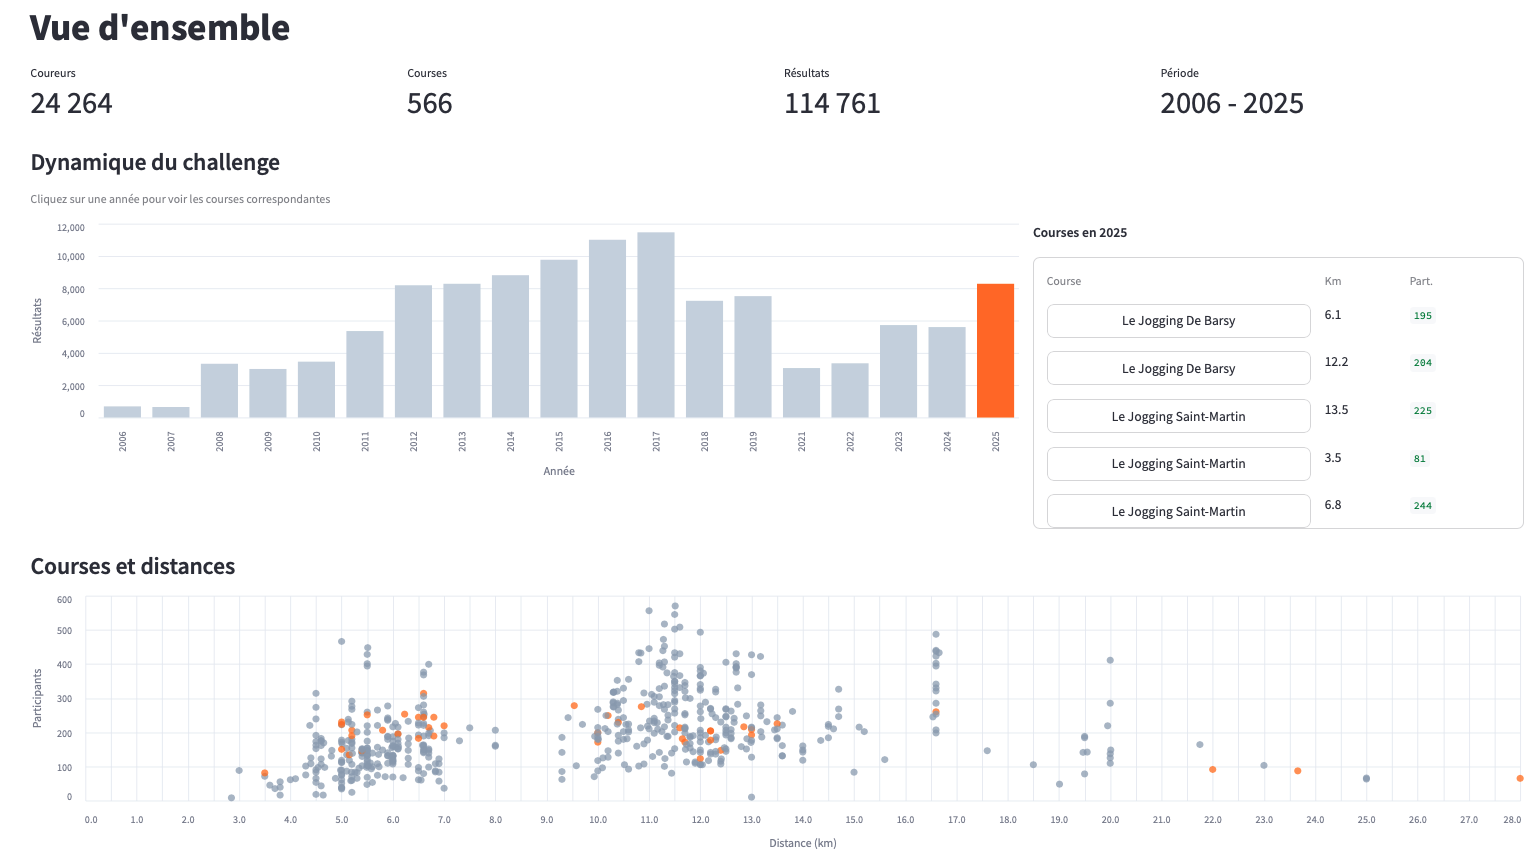
\includegraphics[width=\textwidth]{vue_ensemble.png}
    \caption{Vue d'ensemble de l'application CondruLytics.}
    \label{fig:vue-ensemble-streamlit}
\end{figure}

\subsection{Courses}

La vue par course permet de consulter les résultats détaillés d'une épreuve précise. L'utilisateur choisit d'abord une course parmi les années disponibles. Des indicateurs présentent ensuite le nombre de participants, la distance, le temps moyen et la vitesse moyenne observée sur cette course.

Le premier onglet contient le classement qui reprend les caractéristiques principales. Lorsque des prédictions historiques sont disponibles, le tableau ajoute également le temps attendu et l'écart entre le temps réalisé et le temps attendu. Une valeur négative signifie que le coureur a été plus rapide que ce que le modèle prévoyait. Un filtre par catégorie permet de limiter l'affichage à un groupe précis, ce qui facilite la lecture du classement pour un coureur qui souhaite se comparer à sa catégorie.

L'onglet d'analyse complète le classement avec une lecture globale de la course. Il présente la répartition des participants par catégorie, puis un tableau de synthèse de différentes caractéristiques de la course selon les catégories. 

\begin{figure}[h!]
    \centering
    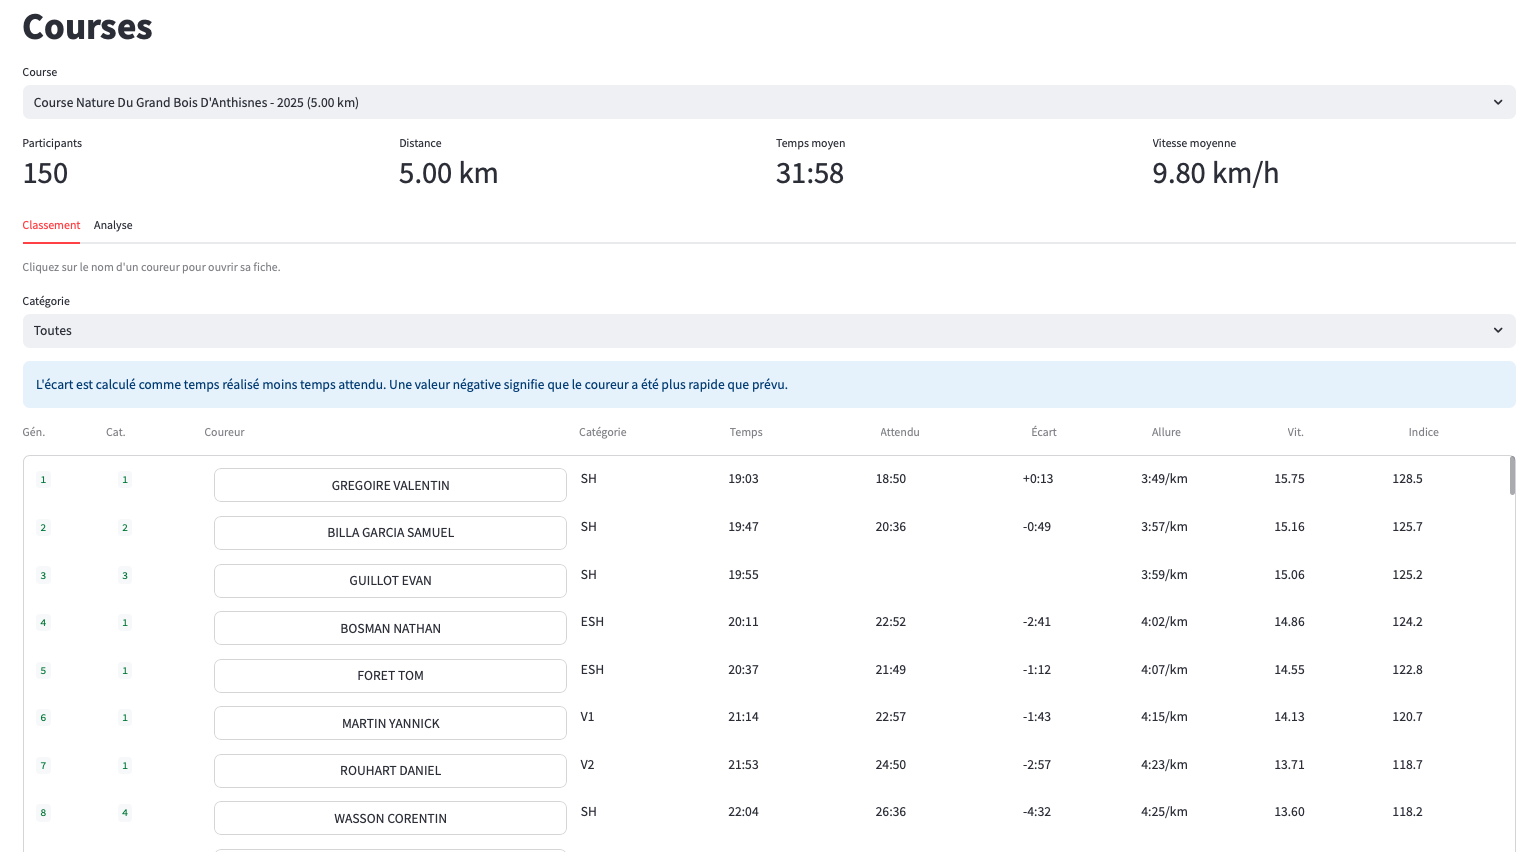
\includegraphics[width=\textwidth]{course_classement.png}
    \caption{Classement détaillé d'une course dans l'application CondruLytics.}
    \label{fig:courses-classement-streamlit}
\end{figure}

\begin{figure}[h!]
    \centering
    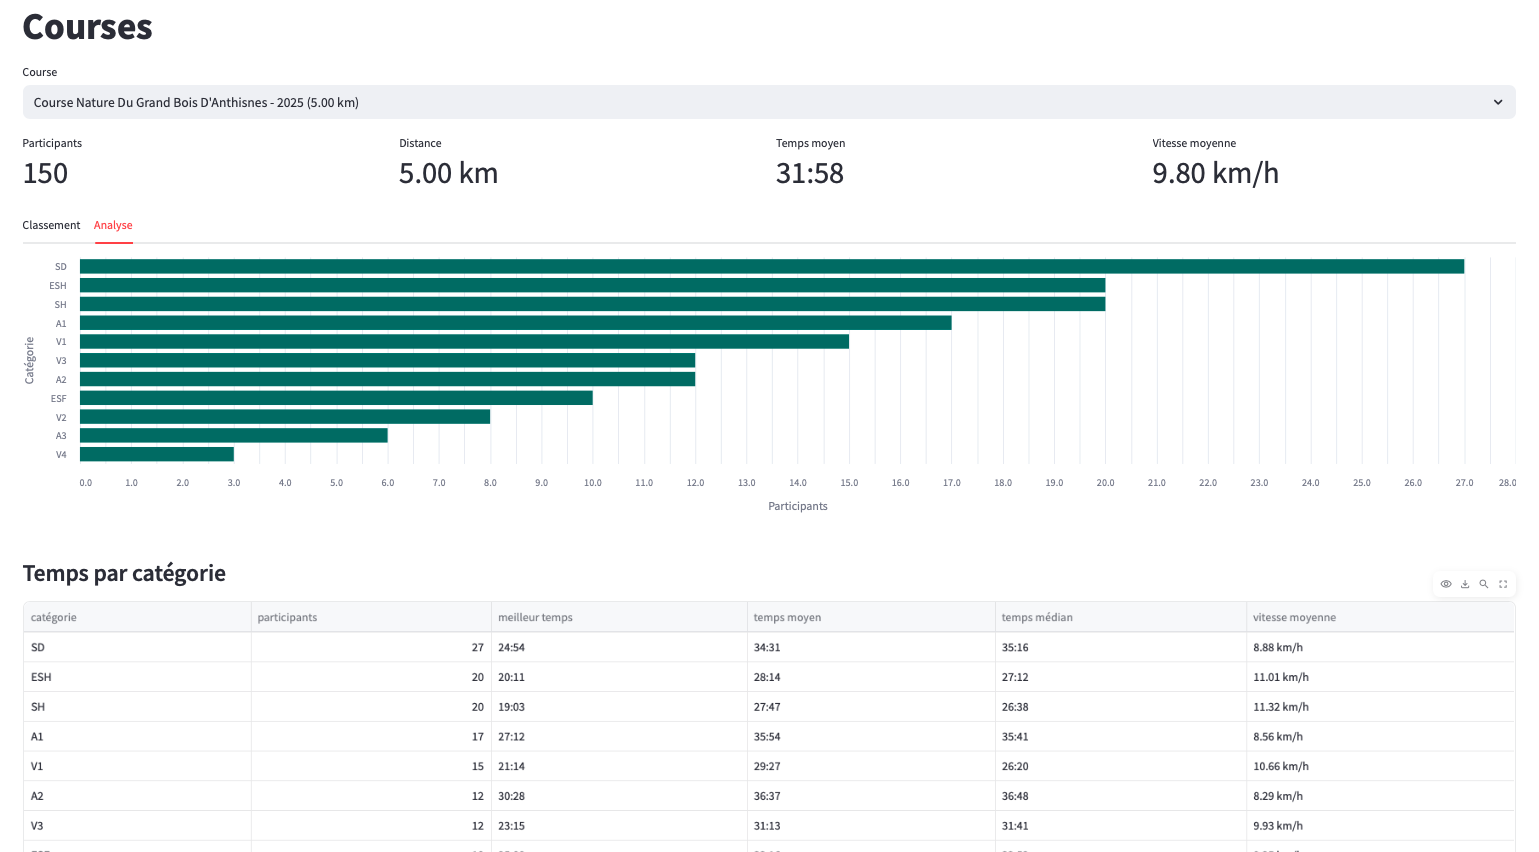
\includegraphics[width=\textwidth]{course_analyse.png}
    \caption{Analyse par catégorie d'une course dans l'application CondruLytics.}
    \label{fig:courses-analyse-streamlit}
\end{figure}

\subsection{Coureurs}

La vue coureur permet d'analyser l'historique individuel d'un participant. Après sélection d'un coureur, l'application affiche quelques indicateurs de synthèse : nombre de courses réalisées, distance totale, allure moyenne, indice moyen et meilleure performance relative.

L'onglet \textit{Profil} présente l'évolution de l'indice de performance au fil du temps. Lorsque les prédictions historiques sont disponibles, l'indice attendu est superposé à l'indice réellement observé, ce qui permet de voir rapidement les courses où le coureur a fait mieux ou moins bien que prévu. Un second graphique donne les performances selon la distance des courses, afin d'analyser la distance de prédilection du coureur.

L'onglet \textit{Simulation} permet d'estimer rétrospectivement le temps qu'un coureur aurait pu réaliser sur une course déjà présente dans l'historique mais qu'il n'a pas courue. L'application affiche alors un temps estimé, une allure, une vitesse et un indice de performance estimé.

Enfin, l'onglet \textit{Détail} reprend l'ensemble des résultats du coureur sous forme de tableau. Le nom de la course est cliquable et permet de revenir à la page détaillée de cette course.

\begin{figure}[h!]
    \centering
    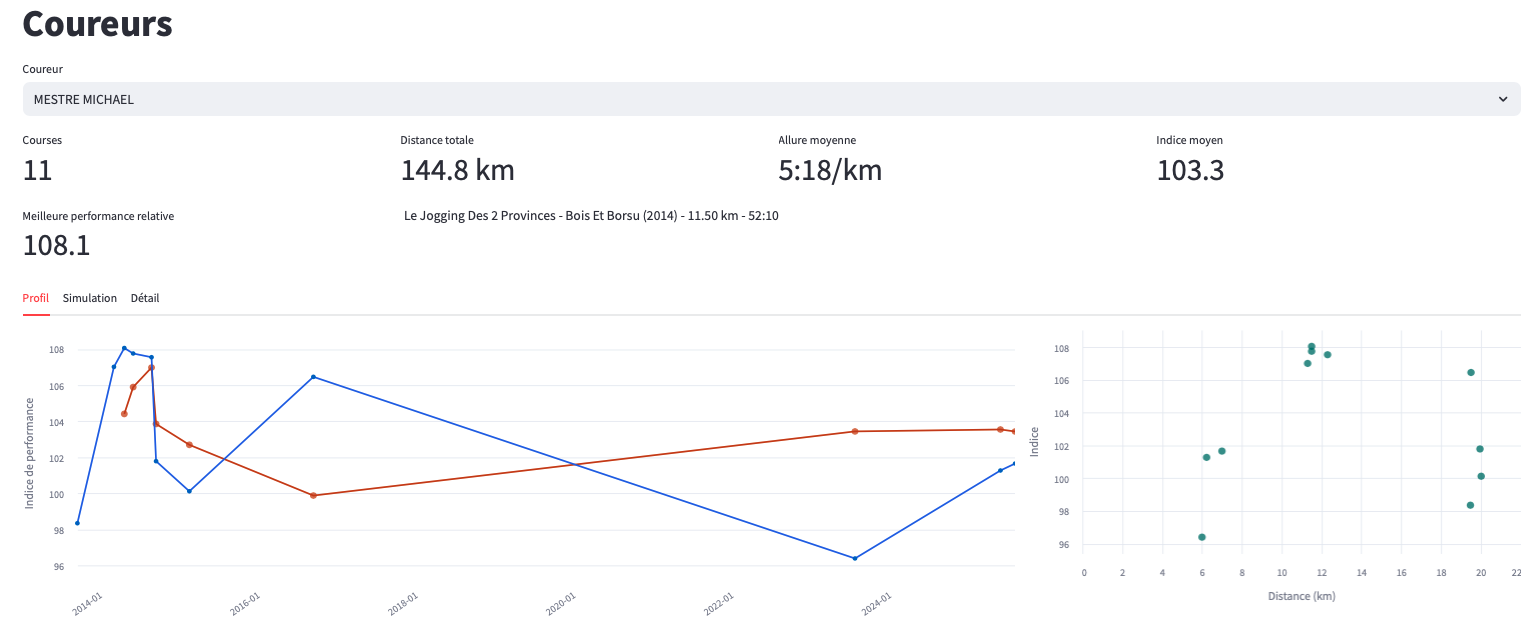
\includegraphics[width=\textwidth]{coureur_profil.png}
    \caption{Profil d'un coureur dans l'application CondruLytics.}
    \label{fig:coureur-profil-streamlit}
\end{figure}

\begin{figure}[h!]
    \centering
    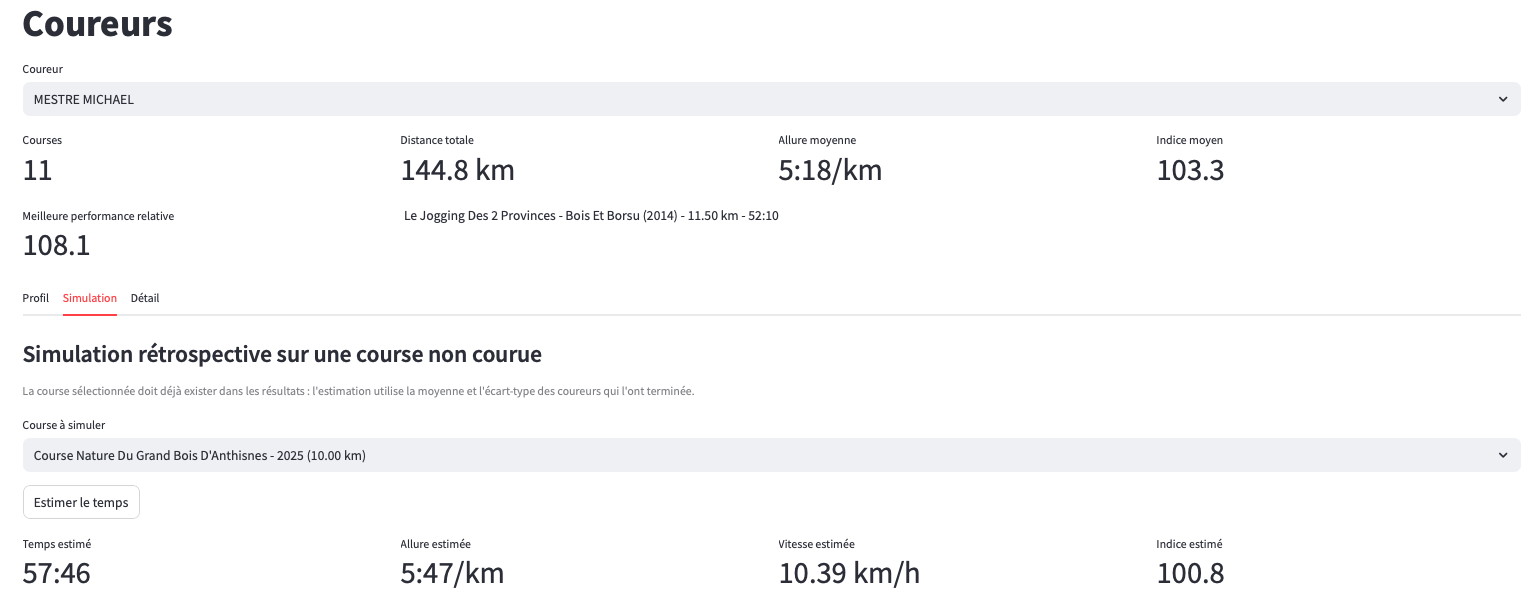
\includegraphics[width=\textwidth]{coureur_simulation.png}
    \caption{Simulation rétrospective d'une course non courue.}
    \label{fig:coureur-simulation-streamlit}
\end{figure}

\begin{figure}[h!]
    \centering
    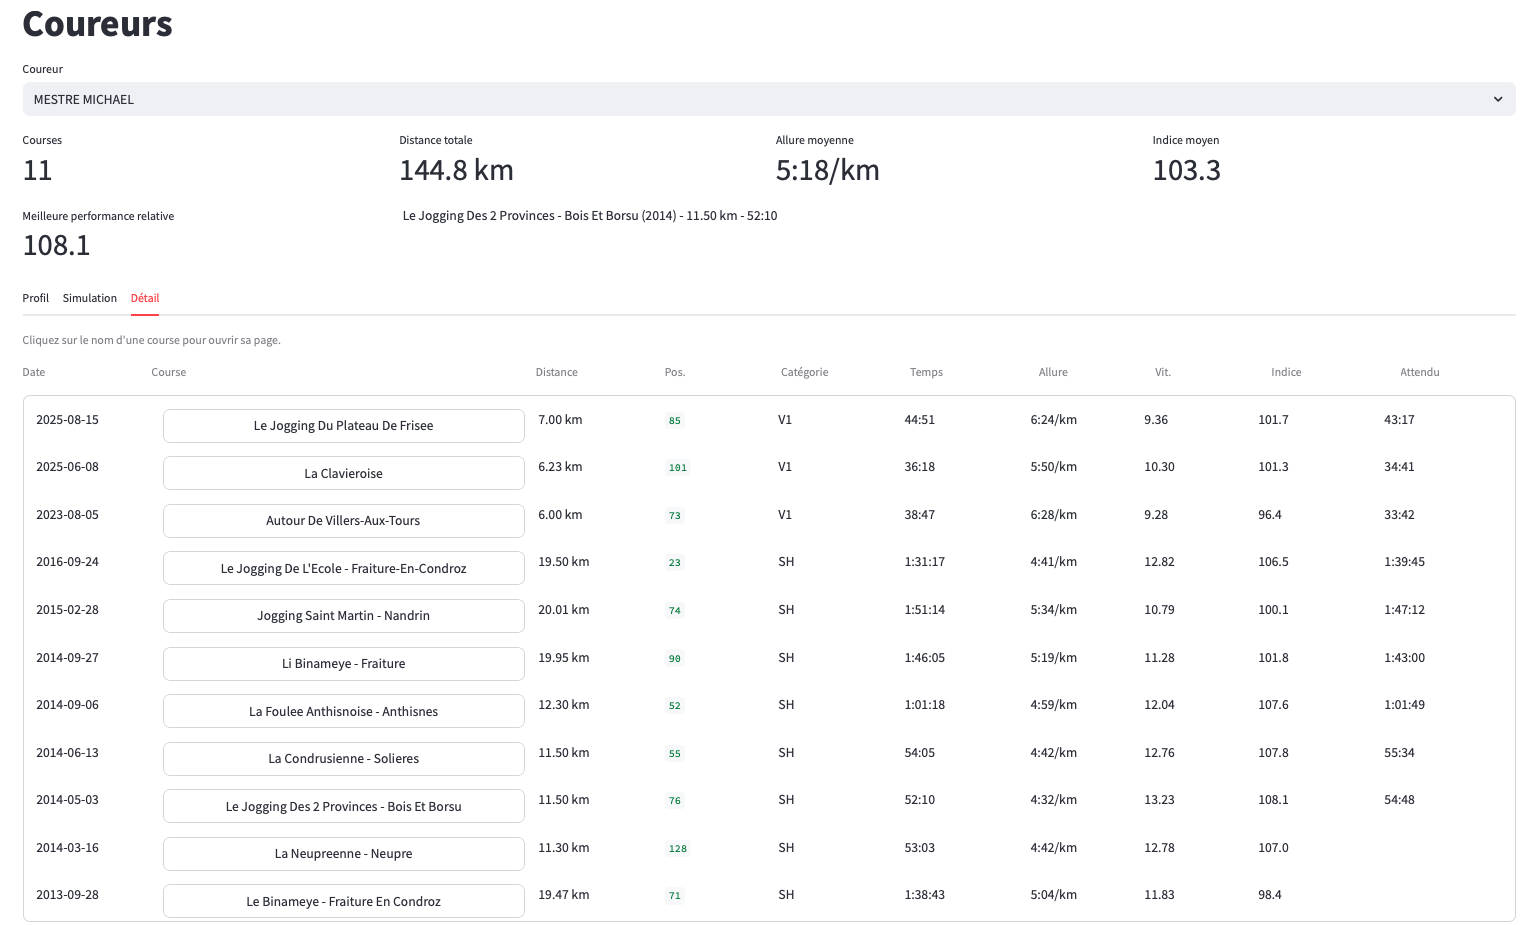
\includegraphics[width=\textwidth]{coureur_detail.png}
    \caption{Détail des résultats d'un coureur.}
    \label{fig:coureur-detail-streamlit}
\end{figure}

\clearpage

\section{Conclusions}

Ce projet part de classements historiques du Challenge Condrusien au format PDF hétérogene pour les transformer en une base de données exploitable et en une application interactive. Cela couvre l'extraction, le nettoyage, la sauvegarde dans une base de données relationnelle, la création de variables, la modélisation prédictive et la visualisation. Son principal objectif est de rendre des données sportives dispersées consultables par course, par coureur et par année, tout en ajoutant des indicateurs de performance et des simulations rétrospectives. Les prédictions doivent cependant etre vues comme une aide a l'analyse, à des suivi de tendance et non comme une mesure définitive de la performance.

\subsection{Limites identifiées}

\begin{itemize}
    \item Les PDF restent hétérogenes, ce qui peut entrainer des erreurs de parsing ou des corrections manuelles.
    \item L'identification des coureurs repose surtout sur le nom nettoyé, avec un risque d'erreur en cas d'homonymes ou de variations d'orthographe.
    \item La simulation est rétrospective : la course cible doit deja exister dans l'historique.
\end{itemize}

\subsection{Perspectives d'amelioration}

\begin{itemize}
    \item Ajouter des tests automatisés sur le parsing, le nettoyage et les transformations.
    \item Améliorer l'identification des coureurs.
    \item Prévoir une strategie pour estimer des courses futures a partir d'éditions précédentes ou de courses comparables.
\end{itemize}

\clearpage

\section*{Références}
\addcontentsline{toc}{section}{Références}

\begin{thebibliography}{1}

\bibitem{openstax_zscore}
OpenStax, ``The Standard Normal Distribution'', \textit{Introductory Statistics}.
\url{https://openstax.org/books/statistics/pages/6-1-the-standard-normal-distribution}

\end{thebibliography}


\end{document}
